\documentclass[a4paper,10pt]{article}
%\usepackage{a4wide}
\usepackage{graphicx}
\usepackage{verbatim}
\usepackage{subfig}
\usepackage{float}
\usepackage[spanish]{babel}
\usepackage[utf8]{inputenc}
\usepackage{tabularx}
\usepackage[left=3.2cm,right=3cm]{geometry}
\hyphenation{des-com-po-ner-los va-rie-dad in-gre-dien-tes ac-tua-li-za-cio-nes me-dian-te con-si-de-ra-cio-nes nues-tro au-to-ma-ti-za-do pro-pues-tos con-tras-ta-das ra-zo-na-ble}

\begin{document}

\tableofcontents

\newpage


\section*{Introducci\'on}
\addcontentsline{toc}{section}{Introducci\'on}
El objetivo de este trabajo es proporcionar la documentaci\'on necesaria para establecer un marco a los objetivos proporcionados por la c\'atedra. Dichos objetivos fueron refinados por los directivos de la cadena Pizza Hack y se presentan en un diagrama, el mismo es considerado un modelo final, es decir que no se presentaban opciones. 

La documentaci\'on a presentar modela comportamientos presentados en el trabajo pr\'actico n\'umero 1.
Para el cumplimiento de este objetivo se tuvo en cuenta la trazabilidad de los modelos proporcionados con los diagramas de objetivos y de contexto recibidos y tambi\'en result\'o importante mantener la trazabilidad entre los distintos modelos realizados a efecto de reflejar de manera eficiente y clara los distintos comportamientos.
Con este fin, se utilizaron diferentes t\'ecnicas de especificaci\'on. A continuaci\'on se establece una introducci\'on a la idea final de cada t\'ecnica:
\begin{itemize}
\item Casos de Uso: Este modelo se utiliz\'o para poder explicar los comportamientos que involucran al mundo y a la m\'aquina, es decir, las que involucran a los humanos, la interacci\'on con la impresora y al servidor de internet para sentar algunos ejemplos.
\item Modelo Conceptual: Este modelo se utiliz\'o para poder mostrar los diferentes componentes que participan para cumplir todos los objetivos finales.
\item Diagrama de Actividad: Este modelo se utiliz\'o para aclarar el comportamiento de algunas secuencias de acciones entre varios actores diferentes.
\item M\'aquina de estados finita: Este modelo se utiliz\'o para poder describir de manera m\'as eficiente el comportamiento del software en algunas actividades que cobran mayor importancia por dentro del mismo.
\end{itemize}

A medida que se vayan realizando los diferentes modelos, se adjuntaran sus explicaciones en base a las decisiones tomadas, as\'i como tambi\'en se mostrar\'a como los diferentes modelos
encajan entre s\'i.

Por \'ultimo, se presentar\'an algunas discusiones y conclusiones finales sobre lo realizado.


\section*{Aclaraciones Generales}
\addcontentsline{toc}{section}{Aclaraciones Generales}

En este trabajo pr\'actico solo se realiz\'o una presunci\'on importante. Al leer los diagramas de objetivos, el diagrama de contexto y los escenarios presentados se pudieron observar algunas inconsistencias, por ejemplo en el diagrama de contexto no existe relaci\'on entre el mozo y el cliente y, sin embargo, los escenarios no indican lo mismo. En estos casos, se decidi\'o seguir la linea de los diagramas y no de los escenarios, aunque cada decisi\'on se encuentra detallada en el cuerpo del trabajo.



\newpage


\section*{Vistas}
\addcontentsline{toc}{section}{Vistas}
En esta secci\'on presentaremos las diferentes especificaciones realizadas durante el presente trabajo pr\'actico.
Se explicar\'a como se abord\'o cada parte del trabajo, explicando para que momentos fue utilizada cada t\'ecnica de especificaci\'on, y el porque
de esta desici\'on.

En un aspecto general, se dividieron las t\'ecnicas de especificaci\'on seg\'un los siguientes crit\'erios:

\begin{itemize}
\item Modelo Conceptual: Se utilizar\'a para un entendimiento global del funcionamiento total de la pizzer\'ia, entiendendo las entidades que interactuan dentro y con el mismo.
\item Diagrama de Casos de Uso: Se utilizar\'a para mostrar todas las interacciones que la m\'aquina tiene con los diversos actores.
\item Diagramas de Actividad: Se utilizar\'an para mostrar secuencias de acciones, usualmente agrupar\'an diversos casos de uso que posean un hilo conductor.
\item M\'aquinas de Estado Finitas: Se utilizar\'an para mostrar las acciones que ocurren principalmente dentro de la m\'aquina para de esta manera, junto a los dem\'as esquemas
, poder dar un panorama completo del comportamiento del software.
\end{itemize}


\bigskip

\subsection*{Modelo Conceptual}
\addcontentsline{toc}{subsection}{Modelo Conceptual}

El modelo conceptual es una primera aproximaci\'on a todo lo que se quiere describir detalladamente en el transcurso de este trabajo. Explica 
de manera temprana la relaci\'on que existe entre los actores externos y las diferentes partes que componen a la pizzer\'ia, para lograr un buen
entendimiento de las interconexiones presentes sin indicar ning\'un tipo de comportamiento por el momento.

A continuaci\'on se presenta el diagrama realizado para este modelo, seguido de las pertinentes explicaciones.

\begin{figure}[H]
\centering
\scalebox{1.1}{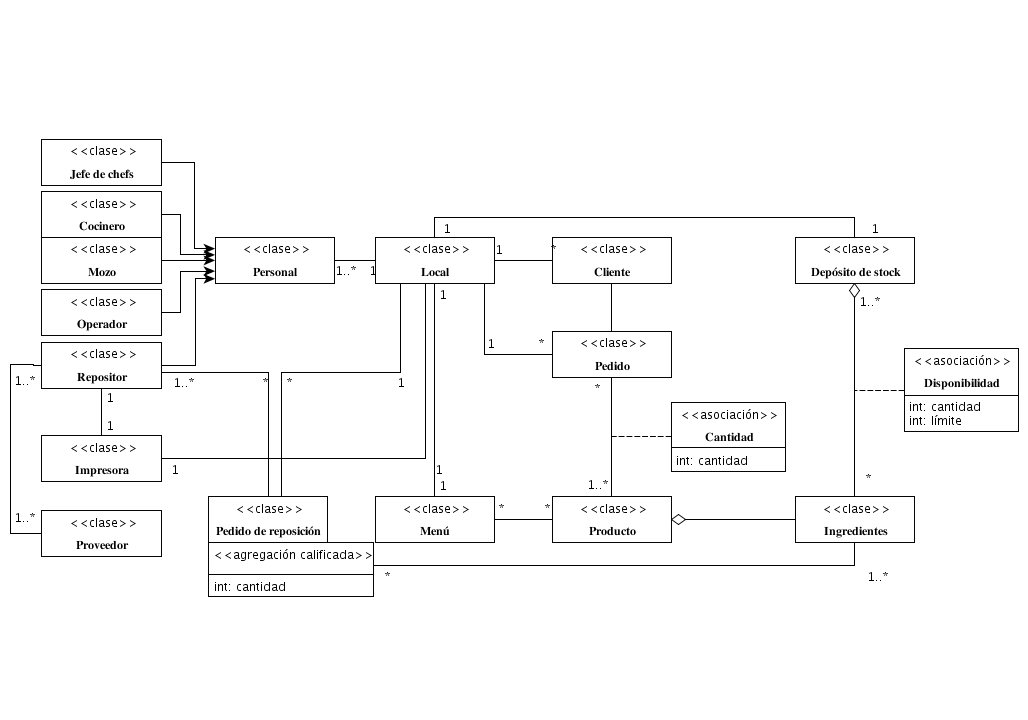
\includegraphics[width=1.0\textwidth]{Imagenes/ModeloConceptual.png}}
\caption{Modelo Conceptual}
\end{figure}

\medskip

Del diagrama anterior se explayan los siguientes puntos para un mejor entendimiento:

\begin{itemize}
\item Dado que hay diferentes cargos dentro del personal se decidi\'o por utilizar el recurso de herencia para identificarlos. Si bien cada subclase
no tiene ning\'un atributo muy distintivo, el repositor tiene algunas relaciones particulares. Este fue el factor determinante para elegir usar herencia
y no poner el tipo de personal como un atributo enumerado, ya que entonces habr\'ia que poner las relaciones del repositor a personal y luego 
restringir por OCL que el relacionado sea de tipo repositor.
\item Por la clase men\'u se entiende el men\'u que la pizzer\'ia ofrece m\'as all\'a del stock que se encuentre disponible.
\item Por la clase producto se entiende cualquier producto que la pizzer\'ia alguna vez ofreci\'o. Esto se realiz\'o de esta manera dado que pensar 
los productos solamente como los que se encuentran en el men\'u podr\'ia traer inconsistencias. Un cliente puede realizar un pedido que contenga un producto
que est\'a en el men\'u (y haya stock para realizarlo), pero una vez hecho este pedido, el producto podr\'ia ser removido del men\'u en una actualizaci\'on,
y a\'un as\'i el pedido con el producto desaparecido del men\'u podr\'ia perdurar en el sistema dado que no se realiz\'o todav\'ia. Es por esto que
pueden existir productos por fuera del men\'u.
\item El cliente esta pensado como una persona o un grupo de personas dentro un local, por eso la multiplicidad cliente-local es uno. Si esa persona
o grupo de personas se movilizacen hac\'ia otro local no hay raz\'on para no pensarlos como un nuevo cliente dentro del otro local.
\item Un pedido de reposici\'on esta conformado por ingrendientes y sus cantidades pedidas, por lo que se opt\'o por utilizar una agregaci\'on calificada
para modelar esto.
\end{itemize}


\medskip

A continuaci\'on se detallar\'an las restricciones sobre el modelo que no se desprenden del diagrama mediante el lenguaje OCL, indicando en cada
caso que fue lo que se quizo restringir en idioma castellano.

\medskip

Se explicitan las correspondencias de cada local con cada tipo de empleado (clase personal y sus subclases).

\medskip

\underline{\textbf{context Local}}

self.personal$\rightarrow$select(p$|$p.isKindOf(Jefe de Chefs)).size()$=1$

self.personal$\rightarrow$select(p$|$p.isKindOf(Cocinero)).size()$>0$

self.personal$\rightarrow$select(p$|$p.isKindOf(Mozo)).size()$>0$

self.personal$\rightarrow$select(p$|$p.isKindOf(Operador)).size()$=1$

self.personal$\rightarrow$select(p$|$p.isKindOf(Repositor)).size()$=1$

\bigskip

\noindent El men\'u es el mismo para todos los locales.

\medskip

\underline{\textbf{context Local}}

Local.allInstances().men\'u$\rightarrow$asSet()$\rightarrow$size()$=1$

\bigskip

\noindent Para todo dep\'osito, cada ingrediente cuyo nivel de stock se encuentre por debajo de mínimo tolerable tiene que estar en un \'unico pedido de reposición relacionado con el local correspondiente al dep\'osito en cuesti\'on.

\medskip

\underline{\textbf{context Depósito de stock}}

self.allInstances()$\rightarrow$select(d$|$d.cantidad$<$d.límite)$\rightarrow$forAll(d$|$d.ingredientes.pedidodereposición.size()$=1$ and d.ingredientes.pedidodereposición$\rightarrow$forAll(p$|$p.local.depósitodestock$=$d.depósitodesotck) 

\bigskip

\noindent Se pide, para un pedido de reposici\'on, una cantidad de stock mayor o igual al límite tolerable de los ingredientes que se encuentran en el pedido de reposición. 
Esto es as\'i para que una vez que se realiza el pedido, seguro se cuente con el m\'inimo necesario.

\medskip

\underline{\textbf{context Ingredientes}}

self.pedidodereposición$\rightarrow$.forAll(p|p.cantidad$\geq$self.disponibilidad.límite)

\bigskip

\noindent La impresora utilizada en un pedido de reposición es la impresora del local que emitió dicho pedido.

\medskip

\underline{\textbf{context Pedido de reposición}}

self.Impresora$=$self.Local.Impresora

\bigskip

\noindent Para todo pedido, el local en donde est\'a ese pedido debe ser el local donde el cliente realiz\'o ese pedido.

\medskip

\underline{\textbf{context Pedido}}

pedido.local $=$ pedido.cliente.local

\newpage

\subsection*{Diagrama de Casos de Uso}
\addcontentsline{toc}{subsection}{Diagrama de Casos de Uso}

Esta t\'ecnica sirve para mostrar como son las interacciones entre el mundo y la m\'aquina, es decir que se abstraen varias de las relaciones presentes
obviando las relaciones prop\'ias entre actores que se encuentran por fuera de la m\'aquina, as\'i como las interacciones que son intr\'insecas de la m\'aquina.

\subsubsection*{Diagrama}
\addcontentsline{toc}{subsubsection}{Diagrama}

A continuaci\'on se presenta el diagrama de casos de uso para toda la m\'aquina, es decir, se engloban todas las interacciones en un mismo diagrama
y luego se detallar\'a en particular cada caso de uso.


\begin{figure}[H]
\centering
\scalebox{1.0}{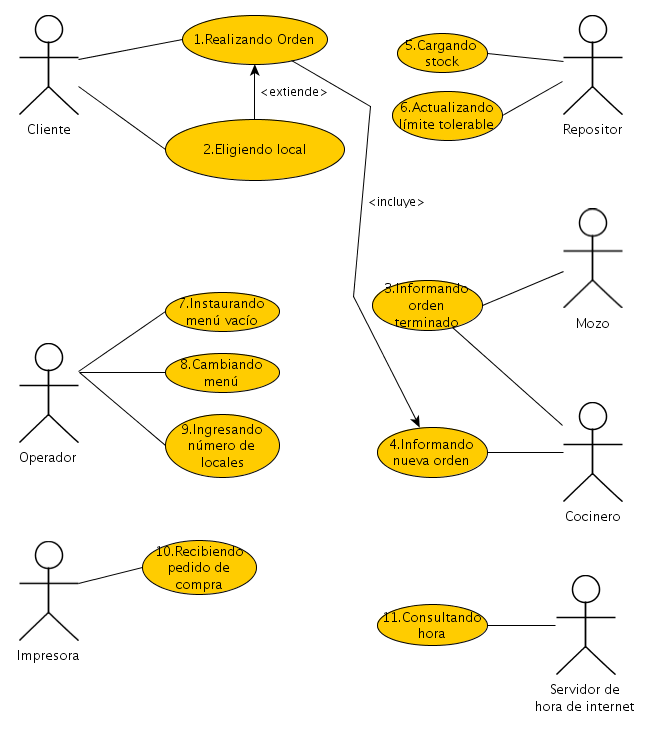
\includegraphics[width=1.0\textwidth]{Imagenes/CasosDeUso.png}}
\caption{Diagrama de Casos de Uso}
\end{figure}


\subsubsection*{Detalles Casos de Uso}
\addcontentsline{toc}{subsubsection}{Detalles de Casos de Uso}

A continuaci\'on se detallar\'a cada caso de uso, dando la descripci\'on de la sucesi\'on de hechos, adem\'as de los actores y la pre y postcondici\'on.

Para seguir un hilo conductor, los casos de uso se encuentran numerados en forma secuencial agrupados por el o los actores participantes.

Se seguir\'a este mismo secuenciamiento para realizar la descripci\'on.

\bigskip


En primer lugar se encuentra unos de los casos de uso m\'as importante en todo el funcionamiento de la pizzer\'ia. La realizaci\'on de un nuevo
pedido por parte del cliente.


\begin{center}
\begin{tabularx}{14cm}{|X|X|}
\hline
\multicolumn{2}{|l|}{Nombre Casos de uso: 1.Realizando orden}\\
\hline
\multicolumn{2}{|l|}{Actores: Cliente}\\
\hline
\multicolumn{2}{|l|}{Precondici\'on: True}\\
\hline
\multicolumn{2}{|l|}{Postcondici\'on: Se logra hacer el pedido}\\
\hline
Curso Normal & Curso Alternativo\\
\hline
1.1 El cliente realiza una orden. & 
\\
\hline
2.1 El sistema verifica que se puede realizar la orden (stock). Si hay stock ir a 3.1, si no hay stock ir a 4.1&
\\
\hline
3.1 El sistema toma el pedido y decrementa el stock debidamente. &
\\
\hline
3.1.1 Se incluye el caso de uso ``Informando nueva orden''. Ir a 5.1 &
\\
\hline
4.1 El sistema notifica que no se puede realizar el pedido. Busca otros locales con stock & Si no hay otros locales con stock ir a 5.1
\\
\hline
4.1.1 Se extiende al caso de uso ``Eligiendo local''. &
\\
\hline
5.1 Fin de caso de uso & \\
\hline
\end{tabularx}
\end{center}


\bigskip

\begin{center}
\begin{tabularx}{14cm}{|X|X|}
\hline
\multicolumn{2}{|l|}{Nombre Casos de uso: 2.Eligiendo Local}\\
\hline
\multicolumn{2}{|l|}{Actores: Cliente}\\
\hline
\multicolumn{2}{|l|}{Precondici\'on: El cliente realiz\'o un pedido que no se puede efectuar en el propio local}\\
\hline
\multicolumn{2}{|l|}{Postcondici\'on: El cliente elige un nuevo local}\\
\hline
Curso Normal & Curso Alternativo\\
\hline
1.1 El cliente recibe una lista de locales donde se puede satisfacer su pedido & 
\\
\hline
2.1 El cliente elige un local de la lista recibida & 2.2 El cliente no eligen ning\'ung local. Ir a 4.1.
\\
\hline
3.1 El software debe informar la nueva orden en el local elegido y decrementa el stock del local elegido. Se incluye Caso de Uso Informando Nueva Orden &
\\
\hline
4.1 Fin Caso de Uso &
\\
\hline
\end{tabularx}
\end{center}

Este caso de uso, en contraste a la mayor\'ia de los dem\'as, contiene una precondici\'on. Este se incluye para imponer una restricci\'on que no
se puede imponer desde el diagrama mismo dado a que no existe expresividad para esto. 

La precondici\'on del caso de uso dice \emph{el cliente realiz\'o un pedido que no se puede efectuar en el propio local}.
Esta precondici\'on se incluye para mostrar que este caso de uso no tiene sentido por si solo sin una precedencia directa del caso de uso
\emph{Realizando Nueva Orden}. Esto no se puede expresar en el diagrama mismo dado que  en la relaci\'on entre los dos casos de uso 
aparece la etiqueta extiende. Esto es as\'i dado que no siempre que se realiza una nueva orden se elige otro local, por lo que no ser\'ia correcta
la inclusi\'on de una etiqueta incluye. Luego, se usa esta precondici\'on para indicar esta restricci\'on y para poder hacer la descripci\'on del caso de uso
ya asumiendo que el cliente realiz\'o una orden que no pudo ser satisfecha en el propio local.

\bigskip

\begin{center}
\begin{tabularx}{14cm}{|X|X|}
\hline
\multicolumn{2}{|l|}{Nombre Casos de uso: 3.Informando Orden Terminada}\\
\hline
\multicolumn{2}{|l|}{Actores: Mozo, Cocinero}\\
\hline
\multicolumn{2}{|l|}{Precondici\'on: Existe una orden en proceso}\\
\hline
\multicolumn{2}{|l|}{Postcondici\'on: Se informa que se finaliz\'o una orden}\\
\hline
Curso Normal & Curso Alternativo\\
\hline
1.1 El cocinero cocina una pizza que se encontraba en una orden en proceso & 
\\
\hline
2.1 El cocinero ingresa en el sistema la finalizaci\'on de la orden pertinente & 
\\
\hline
3.1 El software actualiza el sistema de ordenes, tildando como realizada la orden que el cocinero notific\'o &
\\
\hline
4.1 El software avisa al mozo correspondiente que la orden se encuentra finalizada para retirar &
\\
\hline
5.1 El mozo se entera que se termin\'o una orden y queda dispuesto a ir a buscar la orden para su entrega &
\\
\hline
6.1 Fin Caso de uso &
\\
\hline
\end{tabularx}
\end{center}

\bigskip

\begin{center}
\begin{tabularx}{14cm}{|X|X|}
\hline
\multicolumn{2}{|l|}{Nombre Casos de uso: 4.Informando nueva orden}\\
\hline
\multicolumn{2}{|l|}{Actores: Cocinero}\\
\hline
\multicolumn{2}{|l|}{Precondici\'on: Un cliente realiz\'o un pedido}\\
\hline
\multicolumn{2}{|l|}{Postcondici\'on: El cocinero es informado de la nueva orden a realizar}\\
\hline
Curso Normal & Curso Alternativo\\
\hline
1.1 El software, luego de procesar el pedido del cliente, informa al cocinero sobre la nueva orden & 
\\
\hline
2.1 El cocinero es notificado de la nueva orden y se dispone a su realizaci\'on & 
\\
\hline
3.1 Fin Caso de Uso
\\
\hline
\end{tabularx}
\end{center}


\medskip

Se puede notar que los casos de uso descriptos hasta el momento se encuentran bastante relacionados, dado que todos juntos conforman una secuencia
com\'un de una cena completa de un cliente en un determinado local. Si bien esta relaci\'on es evidente, en el diagrama de casos de uso no se encuentran
en un hilo secuencial dado que esto no es correcto. Desde un punto de vista de casos de usos at\'omicos no ser\'ia correcto relacionar todos los casos de uso
anteriormente descriptos ya que por ejemplo, entre la realizaci\'on de una nueva orden y la informaci\'on de una orden finalizada pueden pasar horas
en el medio y muchos otros sucesos, por lo que no ser\'ia correcto unirlos en el diagrama.


Sin embargo, como la relaci\'on secuencial es notor\'ia, estos casos de uso ser\'an posteriormente agrupados en un diagrama de actividad que muestre
un hilo de ejecuci\'on completo.

\bigskip

\begin{center}
\begin{tabularx}{14cm}{|X|X|}
\hline
\multicolumn{2}{|l|}{Nombre Casos de uso: 5.Cargando Stock}\\
\hline
\multicolumn{2}{|l|}{Actores: Repositor}\\
\hline
\multicolumn{2}{|l|}{Precondici\'on: True}\\
\hline
\multicolumn{2}{|l|}{Postcondici\'on: Se carga el stock en el sistema}\\
\hline
Curso Normal & Curso Alternativo\\
\hline
1.1 El repositor recibe nuevo stock de alg\'un proveedor & 
\\
\hline
2.1 El repositor ingresa al sistema el stock a actualizar & 
\\
\hline
3.1 El software actualiza el stock de los productos que fueron sumados al deposito de ingredientes &
\\
\hline
4.1 Fin Caso de Uso &
\\
\hline
\end{tabularx}
\end{center}


\bigskip

\begin{center}
\begin{tabularx}{14cm}{|X|X|}
\hline
\multicolumn{2}{|l|}{Nombre Casos de uso: 6.Actualizando l\'imite tolerable}\\
\hline
\multicolumn{2}{|l|}{Actores: Repositor}\\
\hline
\multicolumn{2}{|l|}{Precondici\'on: True}\\
\hline
\multicolumn{2}{|l|}{Postcondici\'on: Se actualiza el l\'imite tolerable de alg\'un producto}\\
\hline
Curso Normal & Curso Alternativo\\
\hline
1.1 El repositor decide modificar el l\'imite tolerable de alg\'un ingrediente en particular & 
\\
\hline
2.1 El repositor ingresa al sistema el ingrediente que quiere actualizar y su correspondiente l\'imite actualizado & 
\\
\hline
3.1 El software actualiza el l\'imite tolerable para el ingrediente que fue se\~{n}alado &
\\
\hline
4.1 Fin Caso de Uso &
\\
\hline
\end{tabularx}
\end{center}


\bigskip
Al igual que sucedi\'o con los primeros casos de uso, los casos de uso 5 y 6 tambi\'en se encuentran correlacionados aunque at\'omicamente no lo est\'en.
A su vez, tambi\'en es claro que en una secuencia de acciones del mundo real, estos casos de uso podr\'ian estar relacionados con los casos
de uso 1(realizando orden) y 10(recibiendo pedido de compra). Estas relaciones secuenciales se ver\'an modeladas posteriormente en el diagrama de actividad
referente a todo lo que sucede con respecto al stock cuando se realiza una orden.

\bigskip


\begin{center}
\begin{tabularx}{14cm}{|X|X|}
\hline
\multicolumn{2}{|l|}{Nombre Casos de uso: 7.Instaurando Men\'u vac\'io}\\
\hline
\multicolumn{2}{|l|}{Actores: Operador}\\
\hline
\multicolumn{2}{|l|}{Precondici\'on: True}\\
\hline
\multicolumn{2}{|l|}{Postcondici\'on: Se carga el men\'u vacio en el sistema}\\
\hline
Curso Normal & Curso Alternativo\\
\hline
1.1 El Operador carga un men\'u vac\'io al sistema & 
\\
\hline
2.1 El sistema se actualiza para trabajar con este nuevo men\'u vac\'io & 
\\
\hline
3.1 Fin Caso de Uso &
\\
\hline
\end{tabularx}
\end{center}

\bigskip

\begin{center}
\begin{tabularx}{14cm}{|X|X|}
\hline
\multicolumn{2}{|l|}{Nombre Casos de uso: 8.Cambiando Men\'u}\\
\hline
\multicolumn{2}{|l|}{Actores: Operador}\\
\hline
\multicolumn{2}{|l|}{Precondici\'on: True}\\
\hline
\multicolumn{2}{|l|}{Postcondici\'on: Se actualiza el men\'u}\\
\hline
Curso Normal & Curso Alternativo\\
\hline
1.1 El operador posee una nueva actualizaci\'on para el men\'u & 
\\
\hline
2.1 El operador carga en el sistema la actualizaci\'on & 
\\
\hline
3.1 El software mira el n\'umero de local al que pertenece el operador &
\\
\hline
4.1 El software consulta la hora. Se incluye Casos de uso 11 &
\\
\hline
5.1 El software calcula si el operador se encuentro apto para modificar el men\'u & El operador no se encuentra apt\'o. Ir a 7.1
\\
\hline
6.1 El software actualiza el men\'u &
\\
\hline
7.1 Fin Caso de Uso &
\\
\hline
\end{tabularx}
\end{center}

\bigskip

\begin{center}
\begin{tabularx}{14cm}{|X|X|}
\hline
\multicolumn{2}{|l|}{Nombre Casos de uso: 9.Ingresando n\'umero de locales}\\
\hline
\multicolumn{2}{|l|}{Actores: Operador}\\
\hline
\multicolumn{2}{|l|}{Precondici\'on: True}\\
\hline
\multicolumn{2}{|l|}{Postcondici\'on: Se ingresan los n\'umeros de los locales}\\
\hline
Curso Normal & Curso Alternativo\\
\hline
1.1 El Operador carga el n\'umero de locales & 
\\
\hline
2.1 El sistema actualiza el n\'umero de locales para realizar c\'alculos de round robin & 
\\
\hline
3.1 Fin Caso de uso &
\\
\hline
\end{tabularx}
\end{center}

\bigskip

Los 3 casos de uso anteriormente descriptos son los que m\'as estan relacionados con el hecho de la actualizaci\'on del men\'u. Esto, como ya se
explic\'o con anterioridad, se mostrar\'a de una manera m\'as visual en un diagrama de actividad que muestre lo que sucede al actualizar un men\'u
en el mundo y en la interfaz. Mientras que luego, con una m\'aquina de estados, se modelar\'a lo que sucede dentro de la m\'aquina con esta acci\'on.

\bigskip

\begin{center}
\begin{tabularx}{14cm}{|X|X|}
\hline
\multicolumn{2}{|l|}{Nombre Casos de uso: 10.Recibiendo pedido de compra}\\
\hline
\multicolumn{2}{|l|}{Actores: Impresora}\\
\hline
\multicolumn{2}{|l|}{Precondici\'on: True}\\
\hline
\multicolumn{2}{|l|}{Postcondici\'on: La impresora recibe un nuevo pedido de compra}\\
\hline
Curso Normal & Curso Alternativo\\
\hline
1.1 El software posee uno o muchos ingrendientes que deben ser repuestos & 
\\
\hline
2.1 El software genera el pedido de compra para satisfacer la necesidades calculadas & 
\\
\hline
3.1 El software manda a la impresora la correspondiente orden de compra &
\\
\hline
4.1 Fin Caso de Uso &
\\
\hline
\end{tabularx}
\end{center}

\bigskip

\begin{center}
\begin{tabularx}{14cm}{|X|X|}
\hline
\multicolumn{2}{|l|}{Nombre Casos de uso: 11.Consultando Hora}\\
\hline
\multicolumn{2}{|l|}{Actores: Servidor de hora de internet}\\
\hline
\multicolumn{2}{|l|}{Precondici\'on: Un operador esta intentando actualizar el men\'u}\\
\hline
\multicolumn{2}{|l|}{PostCondici\'on: Se obtiene una actualizaci\'on de la hora}\\
\hline
Curso Normal & Curso Alternativo\\
\hline
1.1 El software requiere la hora para calculos de round robin & 
\\
\hline
2.1 El Software le pide al servidor una actualizaci\'on de la hora & 
\\
\hline
3.1 El Servidor devuelve lo solicitado al software &
\\
\hline
4.1 Fin Caso de Uso &
\\
\hline
\end{tabularx}
\end{center}

\newpage

\subsection*{Diagramas de Actividad}
\addcontentsline{toc}{subsection}{Diagrmas de Actividad}


Los diagramas de actividad son una representaci\'on para mostrar el secuenciamiento de varias acciones que se encuentran relacionadas por alg\'un
hilo conductor. Los diagramas de actividad se encuentran enriquecidos por el hecho de poder soportar varios actores en un mismo hilo mediante la 
separaci\'on por andariveles de las interacciones de cada actor, es por esto que son muy adecuados para modelar las acciones que suceden entre la
m\'aquina y los actores externos e incluso las acciones que suceden entre los actores externos sin interacci\'on con la m\'aquina.

Si bien las interacciones entre el mundo y la m\'aquina ya fueron descriptas en el diagrama de casos de uso, se realiz\'o de forma diferente
ya que la t\'ecnica de casos de uso se basa en centrarse at\'omicamente en cada caso de uso y solo se explicita una relaci\'on entre dos casos de
uso cuando la relaci\'on es inmediata.

En contraposici\'on a los casos de uso, se utilizar\'an los diagramas de actividad para modelar las secuencias de acciones que sucederi\'an en la 
pizzer\'ia, sin centrarse en cada paso de la secuencia particularmente (dado que ya fueron explayados en los casos de uso).

Se decidi\'o que la t\'ecnica ser\'ia utlizada para los siguientes casos particulares:

\begin{itemize}
\item El ciclo de vida completo de una orden.
\item Ejemplo de manejo de stock.
\item Actualizaci\'on del men\'u.
\end{itemize}


\subsubsection*{Ciclo de vida de una orden}
\addcontentsline{toc}{subsubsection}{Ciclo de vida de una orden}

Este diagrama de actividad sirve para agrupar las acciones sucecidas en el ciclo de vida de una orden, es decir desde el momento que un cliente
pide una orden hasta el momento que recibe su pizza(o bien no la recibe porque no se puede satisfacer). Cabe destacar que en el diagrama de actividad
se abstraen varias situaciones para centrarse solamente en la orden en s\'i. Es decir, si bien usar los ingrendientes para realizar una orden podr\'ia
desencadenar un pedido al proveedor, no ser\'a modelado en este diagrama, sino en el siguiente.

En este diagrama se destaca la diferencia entre que el pedido se cocine en el local donde el cliente se encuentra o en otro, por lo que se 
diferencian entre el cocinero y el mozo del local propio y el cocinero y el mozo del local externo donde el cliente va a ir a buscar la pizza.

\begin{figure}[H]
\centering
\scalebox{1.0}{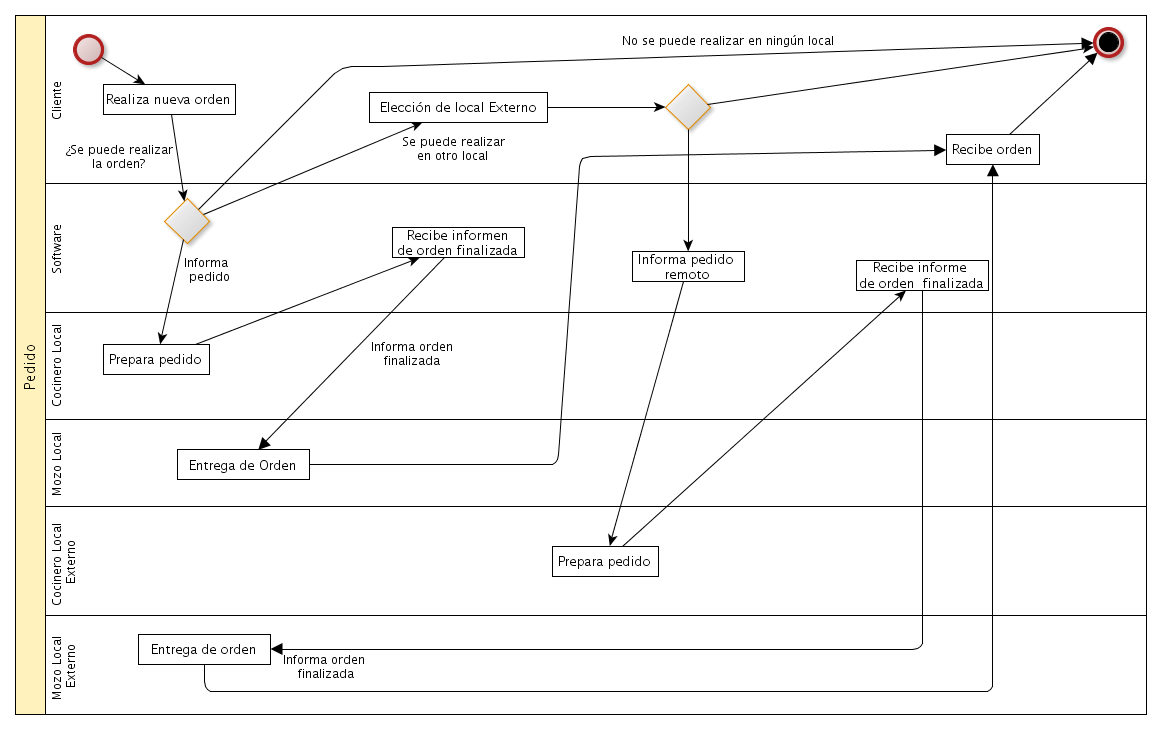
\includegraphics[width=1.0\textwidth]{Imagenes/DA-Pedido.png}}
\caption{Ciclo de vida de una orden}
\end{figure}

\bigskip

\subsubsection*{Ejemplo de manejo de stock}
\addcontentsline{toc}{subsubsection}{Ejemplo de manejo de stock}

Este diagrama de actividad se utilizar\'a para modelar las acciones pertinentes al manejo de stock cuando se realiza una orden. Dado que solo
se quiere modelar lo relacionado con el stock, ya que los otros aspectos respectivos a la realizaci\'on de una orden fueron modelados anteriormente,
el diagrama presenta una secuencia de acciones donde un cliente realiza una orden que se puede satisfacer por dicho local para poder mostrar concretamente
que sucede con el stock sin p\'erdida de generalidad.

\begin{figure}[H]
\centering
\subfloat{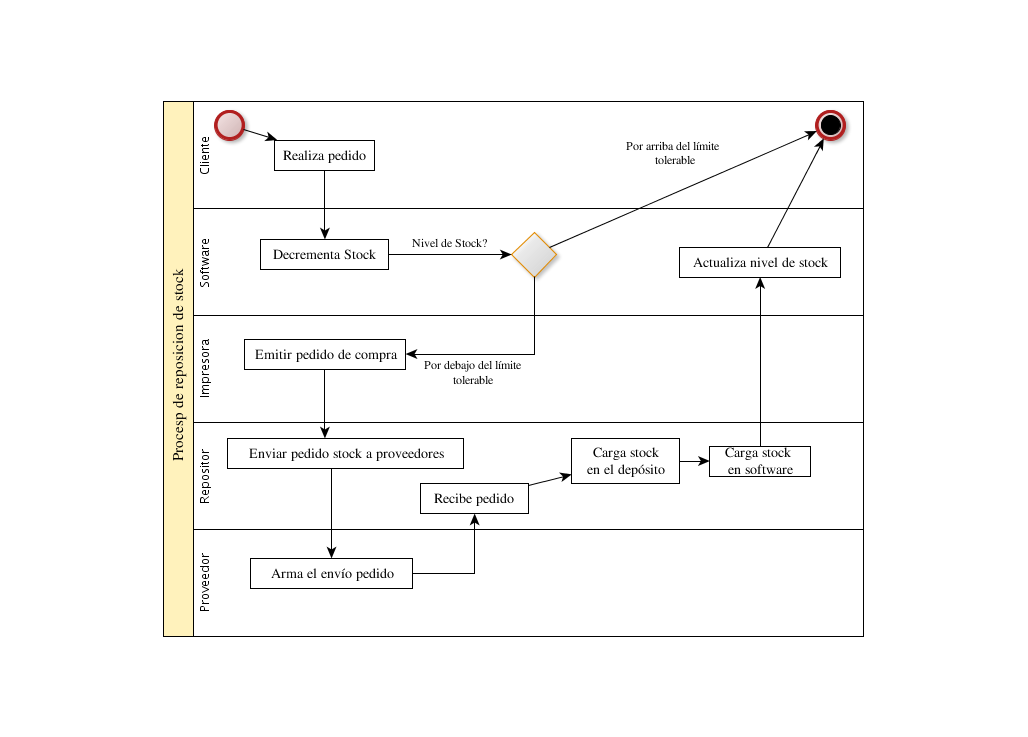
\includegraphics[width=1.0\textwidth]{Imagenes/DA-ReposicionStock.png}}
\caption{Ejemplo de manejo de stock}
\end{figure}

\bigskip

\subsubsection*{Actualizaci\'on del men\'u}
\addcontentsline{toc}{subsubsection}{Actualizaci\'on del men\'u}

Este diagrama de actividad sirve para modelar el hilo de ejecuci\'on de las acciones referidas a la actualizaci\'on de un men\'u en cuanto a la interacci\'on
de los actores externos participantes con la m\'aquina. Lo que sucede dentro de la m\'aquina para mantener una consistencia entre los locales es inherente
a la m\'aquina misma por lo que ser\'a modelado posteriormente con la t\'ecnica de m\'aquinas de estados.

\begin{figure}[H]
\centering
\subfloat{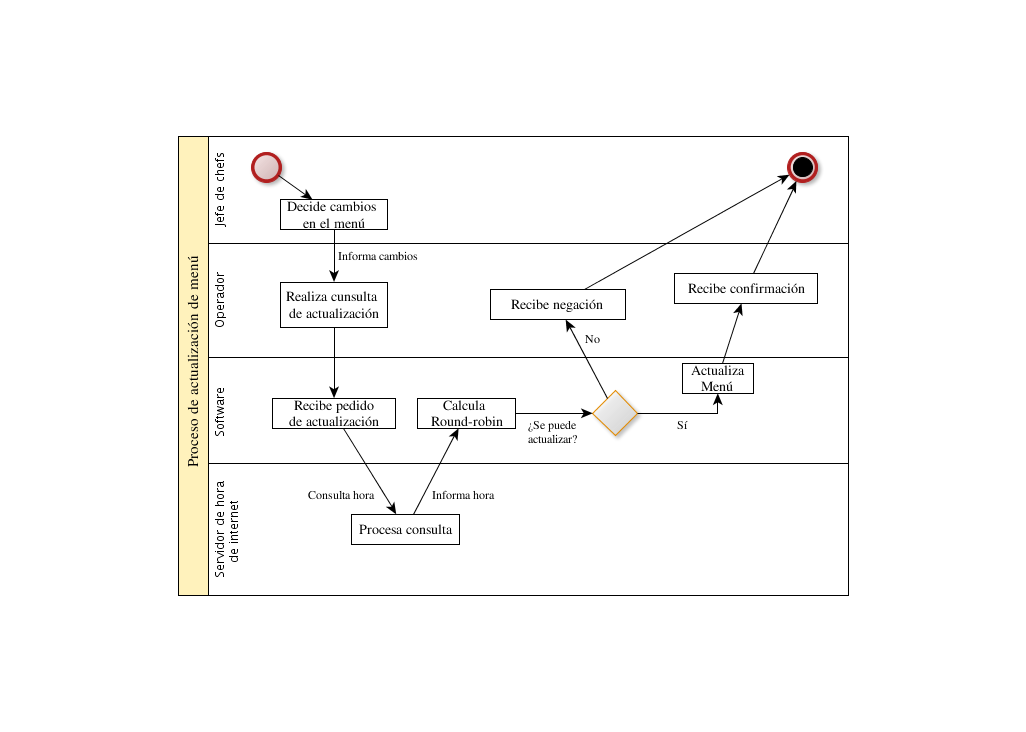
\includegraphics[width=1.0\textwidth]{Imagenes/DA-ActualizacionMenu.png}}
\caption{Actualizaci\'on del men\'u}
\end{figure}


\bigskip

\subsection*{M\'aquinas de Estados Finitas}
\addcontentsline{toc}{subsection}{M\'aquinas de Estados Finitas}

Las m\'aquinas de estados finitas son importantes en este trabajo pr\'actico para poder modelar las acciones que suceden totalmente dentro del software. En este trabajo en particular hay muchas interacciones entre el software y los agentes externos y no existen tantas acciones dentro del mismo que necesiten de una explicaci\'on con m\'aquinas de estado, por lo que este modelo se utilizar\'a en pocos casos. 

En particular en este trabajo, esta t\'ecnica se utiliz\'o para modelar dos aspectos que son relevantes al software por dentro, siendo dignos de una explicaci\'on m\'as hexaustiva. Por un lado se explicar\'a el proceso de actualizaci\'on de men\'u, viendo como se realiza la sincronizaci\'on entre los diferentes locales. Por otro lado, se utilizar\'a la t\'ecnica para explicar como el software puede revisar el stock de otros locales para derivar el pedido de un cliente.


\subsubsection*{Sincronizaci\'on del men\'u}
\addcontentsline{toc}{subsubsection}{Sincronizaci\'on del men\'u}

En esta m\'aquina de estados se explicar\'an los cambios internos del software a respuesta de los est\'imulos externos. Para modelar los est\'imulos externos se realizar\'an m\'aquinas de estados por cada agente externo que interactue con el sistema.

A continuaci\'on se ir\'an explicando cada agente, para llegar a la explicaci\'on final del accionamiento del software.
El \'indice i en cada m\'aquina de estados, va desde 1 hasta la cantidad de locales y hace referencia al n\'umero del local.

\noindent \underline{Jefe de chefs}:

\begin{figure}[H]
\centering
\scalebox{0.5}{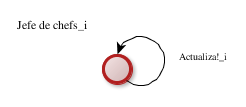
\includegraphics[width=1.0\textwidth]{Imagenes/JefedeChefs.png}}
\caption{Jefe de Chefs}
\end{figure}

El accionar del jefe de chefs es muy simple, cuando tenga ganas va a querer actualizar y esto es lo \'unico significante que hace. Esta acci\'on tendra que ser \emph{escuchada} por el operador de su propio local.

\bigskip

\noindent \underline{Servidor de hora de internet}:

\begin{figure}[H]
\centering
\subfloat{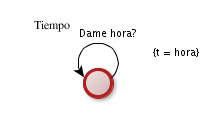
\includegraphics[width=1.0\textwidth]{Imagenes/Servidor.png}}
\caption{Servidor de hora}
\end{figure}

El accionar del servidor de hora tambi\'en es simple, solamente esta dispuesto a escuchar una acci\'on que es que le pidan la hora, cuando esta sucede, setea el tiempo en la hora actual del d\'ia. Es el mismo servidor por todos los locales por eso no tiene diferenciaci\'on de \'indice ni en el nombre del servidor, pero si tiene \'indice la transicion para no forzar que todas las m\'aquinas pidan hora al mismo tiempo.

\bigskip

\noindent \underline{Operador}: 

\begin{figure}[H]
\centering
\subfloat{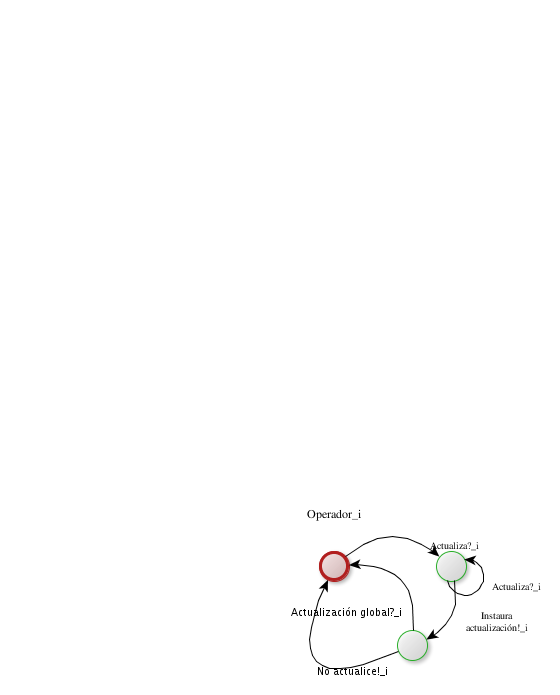
\includegraphics[width=1.0\textwidth]{Imagenes/Operador.png}}
\caption{Operador}
\end{figure}

El Operador ya tiene algunas acciones que merecen una explicaci\'on m\'as detallada. Por un lado el operador debe escuchar la acci\'on de actualizar generada por su propio jefe de chefs, luego una vez que posee una actualizaci\'on del jefe de chefs, busca instaurar esta actualizaci\'on en el software del local, generando la acci\'on \emph{Instaura actualizacion}. Aqu\'i el Operador, pasa a un estado intermedio donde espera a que el software le diga si se pudo instaurar globalmente la actualizaci\'on o si no se pudo. Durante este estado, el Operador no escucha actualizaciones de su jefe de chefs. Adem\'as cabe destacar que si el software no le da permiso al operador para instaurar la actualizaci\'on esta actualizaci\'on se pierde y el jefe de chefs debe volver a generarla. Estas fueron decisiones tomadas por el grupo, ya que no se especifica como debe ser esto ni en los objetivos ni en el diagrama de contexto, por lo que qued\'o a criterio del grupo.

\bigskip

\noindent \underline{SoftwareLocal}:

\begin{figure}[H]
\centering
\subfloat{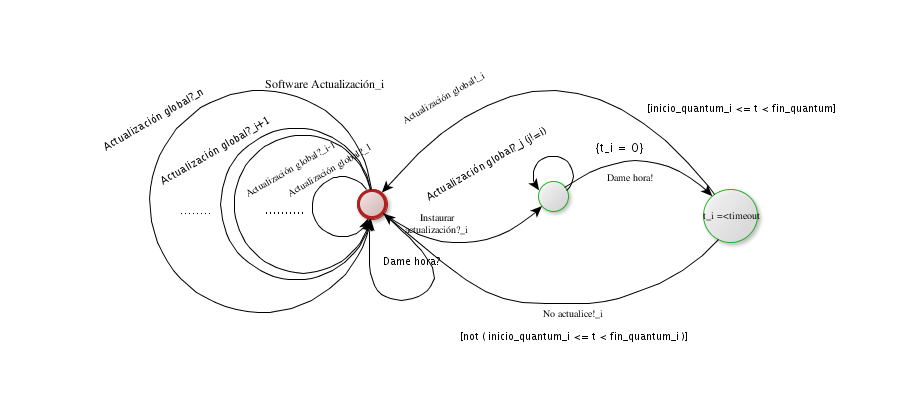
\includegraphics[width=1.0\textwidth]{Imagenes/SoftActualizacion.png}}
\caption{Software}
\end{figure}


El software comienza en un estado inicial donde lo que tiene permitido hacer es escuchar las actualizaciones globales de los otros locales o, por otro lado, esperar un pedido de instauraci\'on de actualizaci\'on de su propio operador. Una vez que su operador le pide instaurar una actualizaci\'on, el software pasa a un estado donde va a querer hacer una actualizaci\'on. En este estado el software pide la hora al servidor para saber si es su momento para actualizar o no. Si es su momento, despues de un timeout el software \emph{saldr\'a} por la transici\'on superior, generando una actualizaci\'on global que sera escuchada por los dem\'as locales. En caso de no ser su momento, no realizar\'a su actulizaci\'on volviendo al estado inicial.



\subsubsection*{Pedido a distancia}
\addcontentsline{toc}{subsubsection}{Pedido a distancia}

En un pedido a distancia solo se presentar\'an dos diferentes m\'aquinas de estado, una por el cliente de un local y otra por el software de cada local. Para simplicidad del modelo se asume que un solo cliente por local esta involucrado por vez en este proceso.

A continuaci\'on se presenta la m\'aquina de estados del cliente.

\begin{figure}[H]
\centering
\subfloat{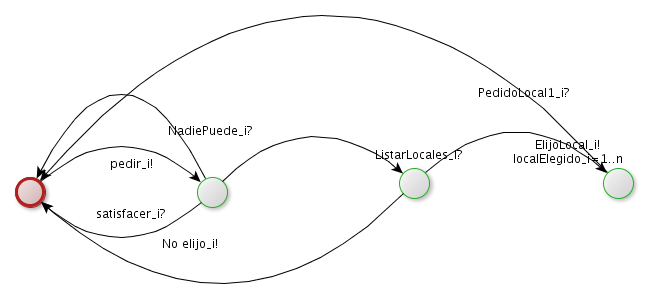
\includegraphics[width=1.0\textwidth]{Imagenes/Cliente.png}}
\caption{Cliente}
\end{figure}

El cliente empieza en un estado inicial en donde lo que puede hacer es pedir una pizza, si la pizza puede ser hecha por el mismo local o si ningun local puede satisfacerlo, el cliente vuelve al estado inicial ya sea satisfecho o no, pero sin nada m\'as que hacer en esta secuencia. Por otro lado, el software puede presentarle una lista de locales para elegir y el cliente pasa a un estado de elecci\'on. Si no elige ning\'un local, termina el proceso. Si, por el contrario, elige un local, pasara a un estado donde se generara el pedido al otro local terminando el proceso.


Luego, se presenta la m\'aquina de estados del software de cada local.
Antes que nada cabe destacar que en todo nodo la fsm esta \emph{escuchando} el pedido StockTodos de las demas maquinas as\'i como tambi\'en los pedidoslocal de las dem\'as m\'aquinas que les mandan pedidos, lo cual se omite para una mayor claridad del dibujo ya que no aporte mayor informaci\'on m\'as que la idea intuitiva que un local siempre tiene que estar dispuesto a recibir un pedido de otra m\'aquina o a que le pidan su stock.

\begin{figure}[H]
\centering
\subfloat{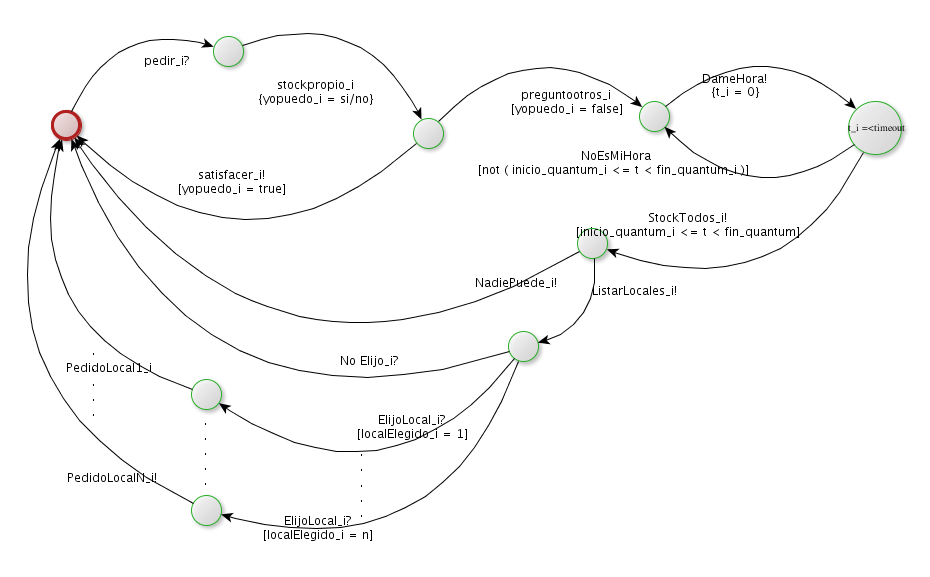
\includegraphics[width=1.0\textwidth]{Imagenes/FSMpedidoadistancia.png}}
\caption{Software}
\end{figure}

La m\'aquina comienza en un estado inicial donde lo \'unico que hace es escuchar el pedido de un cliente. Luego de que un cliente hace un pedido, el software va a revisar su stock propio y se va a setear la variable yopuedoi en base a si puede satisfacer el pedido o no. Si puede satisfacerlo, lo satisface y vuelve al estado inicial esperando por otro cliente. Si no puede, pasara a un estado para preguntar por los otros. Aqui el software pide la hora para saber si esta en su quantum, con una soluci\'on an\'aloga a la propuesta en la m\'aquina de estados para actualizar el men\'u. Una vez que esta en su hora, genera una transicion denominada, StockTodosi! que sera escuchada por todas las maquinas, que indicar\'an si pueden realizar el pedido en cuesti\'on. Si nadie puede satisfacer el pedido, el software vuelve al estado inicial a esperar por otro cliente. Si existen otros locales que puedan hacer el pedido, el software se los lista al cliente.

Aqu\'i pueden pasar dos cosas. En primer lugar, el cliente podr\'ia no elegir ning\'un local a distancia por lo que se vuelve al estado inicial. Por otro lado, el cliente puede elegir un local y setear la variable localelegidoi, de esta manera el software saldra por la unica transici\'on que tenga la condici\'on true, llegando a un estado donde lo que va a hacer es generar un pedido externo al local correspondiente.

De esta manera, se genera todo el ciclo posible en un pedido a distancia, mostrando la funcionalidad del software en funci\'on de los requisitos del cliente.




\newpage


\section*{Discusi\'on}
\addcontentsline{toc}{section}{Discusi\'on}

Durante el desarrollo del presente trabajo pr\'actico, se fue explicando en cada momento el porque de la elecci\'on de las diferentes
t\'ecnicas de modelado en cada uso en particular. Dicha decisi\'on es en parte arbitraria y en parte no, es decir hubo decisiones que estuvieron
influenciadas por la naturaleza de las t\'ecnicas en s\'i mismas mientras que hubo otras desiciones que fueron m\'as all\'a de las t\'ecnicas
y que tuvieron que ver con la expresividad que se le quizo dar a cada parte del trabajo en particular. Con lo anteriormente dicho, lo que se quiere notar
es que hubo partes de la soluci\'on donde no hubo decisiones personales, por ejemplo la t\'ecnica de casos de uso sirve para modelar las interacciones
entre el mundo y la m\'aquina y eso no fue una desici\'on del grupo, mientras que la cantidad y la especificidad de los diagramas de actividad
y las m\'aquinas de estado, si fueron una decision tomada por el grupo.

En lo siguiente, se ver\'a porque las decisiones se tomaron de esta manera, explicando como estas decisiones logran que la conjuci\'on
de los modelos prediquen sobre todos los aspectos necesarios expuestos en los diagramas de objetivo y en el diagrama de contexto.

\subsection*{Diagrama de Contexto}
\addcontentsline{toc}{subsection}{Diagrama de Contexto}
Se puede ver que el diagrama de contexto se encuentra explicado en su totalidad por los diferentes modelos que se explayaron en este trabajo pr\'actico.

Por un lado, el diagrama de Casos de Uso modela todas las interacciones que existen entre la m\'aquina y el mundo. Es decir, cada caso uso explica
at\'omicamente cada una de las relaciones presentes entre un actor externo y el software, como por ejemplo la interacci\'on que existe entre
el cocinero y el software, cuando el primero le avisa al segundo que la orden fue finalizada. 

Dada la naturaleza de la t\'ecnica, quedan por fuera de la misma, las interacciones presentes entre los actores externos en los que la m\'aquina
no tiene participaci\'on. 

Para resolver esto, se utilizaron los diferentes diagramas de actividad. Basicamente, se puede notar, que cada una de las relaciones del diagrama de
contexto se puede categorizar en una o m\'as de las 3 siguientes categorias:
\begin{itemize}
\item Las relaciones que tienen inferencia en una orden de un producto.
\item Las relaciones que tienen inferencia sobre el manejo adecuado del stock de la pizzer\'ia.
\item Las relaciones que tienen inferencia sobre la actualizaci\'on y el correcto mantenimiento del men\'u.
\end{itemize}

Es por esto, que se decidi\'o realizar tres diferentes diagramas de actividad, para englobar las diferentes acciones y mostrar as\'i como 
estan relacionadas en el mundo real, aspecto que se escapaba de los casos de uso, debido a su atomicidad.



Por otro lado, el modelo conceptual tambi\'en aporta a la explicaci\'on del diagrama de contexto, aunque como ya se mencion\'o, su aporte
es un poco m\'as transversal a todos los objetivos y al diagrama de contexto, dando una visi\'on m\'as general.


Por \'ultimo, cabe destacar que las m\'aquinas de estado no realizaron un mayor aporte a la explicaci\'on de este diagrama, dado que estan m\'as bien
centradas en lo que sucede dentro del software.

\subsection*{Diagramas de Obejetivos}
\addcontentsline{toc}{subsection}{Diagramas de Objetivos}

\subsubsection*{Pedido a distancia}
\addcontentsline{toc}{subsubsection}{Pedido a distancia}

Este objetivo se centra en el hecho de poder pedir a distancia, pero si vemos las refinaciones vemos que este diagrama se centra en el hecho de las acciones internas que deben ocurrir para esto, ya que toda hoja esta asignada al software. Es por esto, que este objetivo se explica con una m\'aquina de estado, ya que muestra que pasa con el software por dentro para lograr un pedido a distancia.

 
\subsubsection*{Mantener men\'u estandar}
\addcontentsline{toc}{subsubsection}{Mantener men\'u estandar}

El objetivo de mantener un men\'u estandar posee un refinamiento en tres subobjetivos. Por un lado se encuentra el simple objetivo referente
al men\'u vacio, este objetivo no tiene complejidad y se encuentra descripto en un caso de uso que hace referencia a esta acci\'on at\'omica.

Por otro lado, los otros dos subobjetivos si presentan una complejidad mayor y tratan sobre el aspecto m\'as importante, que es como lograr una 
correcta sincronizaci\'on. Los comportamientos del sistema referentes a la satisfabilidad de estos subobjetivos se encuentran explicados de dos maneras
diferentes: Por un lado existe un diagrama de actividad que explica lo que sucede por fuera de la m\'aquina, es decir explica lo que sucede entre todos
los actores que tienen que ver en esta acci\'on, y por el otro se encuentra una m\'aquina de estados que muestra lo que sucede dentro del software
mismo, al momento de querer lograr estos subobjetivos.

\subsubsection*{Nivel adecuado de stock}
\addcontentsline{toc}{subsubsection}{Nivel adecuado de stock}

Este objetivo se encuentra abordado de diferentes maneras tambi\'en. Se encuentra explicado mediante los casos de uso que hacen referencia a la 
interacci\'on entre la m\'aquina y los diferentes actores que tiene influencia en la variabilidad del stock como el repositor y el cliente, y 
tambi\'en por los actores que son influenciados por la variabilidad del stock, como podr\'ia ser la impresora.

Adem\'as se puede encontrar un diagrama de actividad que modela toda una secuencia que podr\'ia suceder en el mundo real, mostrando como 
esta secuencia se relaciona con el stock.

\subsubsection*{Brindar servicios del men\'u}
\addcontentsline{toc}{subsubsection}{Brinda servicios del men\'u}

Este objetivo se encuentra refinado en dos subobjetivos que predican sobre poder realizar una orden, o impedir que se realice si no se puede.
Estos subobjetivos se encuentra explicados por diferentes partes del trabajo pr\'actico. Por una lado, todo lo referente a stock esta bastante
ligado al objetivo anterior y, por ende, se encuentra explicado en el diagrama de actividad mencionado anteriormente, y en los casos de uso correspondientes.
Mientras que todo lo referente al pedido de una orden en s\'i y lo que sucede con ella se encuentra tambi\'en explicado de dos formas diferentes.
Por un lado se tienen los casos de uso at\'omicos inherentes a cada parte de la acci\'on total de pedir una pizza y recibirla, ejemplos de esto
podr\'ian ser los casos de uso Informando nueva orden y eligiendo local. Por otro lado, se tiene un diagrama de actividad espec\'ifico para el
ciclo de vida de una orden que muestra como interactuan todas las partes y las diferentes alternativas que se pueden presentar.


\newpage
\section*{Conclusiones}
\addcontentsline{toc}{section}{Conclusiones}


Luego de finalizar con los modelos presentados en este trabajo, se lleg\'o a varias conclusiones.

En primer lugar se encontr\'o un gran contraste entre el primer trabajo pr\'actico y el segundo.
En el primer trabajo el enunciado era bastante vago y ambiguo debido a que se describ\'ia una situaci\'on coloquial. Esto
trajo aparejado el hecho de que la principal acci\'on del grupo fue tomar una gran cantidad de decisiones y fundamentar las diferentes
alternativas posibles, en los cuales los modelos a utilizar no eran muy restrictivos. Por otro lado, en este segundo trabajo pr\'actico el grupo se encontr\'o
con una aproximaci\'on m\'as formal, por lo que la mayor\'ia de las decisiones fueron sobre cual modelo utilizar para explicar cada parte de lo
entregado por la c\'atedra, pero una vez realizado esto el trabajo tuvo m\'as que ver con la correcta utilizaci\'on de las t\'ecnicas (sus sintaxis, sus restricciones)
y no con presentar alternativas, ya que estas ya habia sido podadas entre el primer trabajo y los supuestos directivos de la pizzer\'ia.

En segundo lugar, se concluye en que las etapas al encarar el trabajo fueron satisfactorias aunque se podr\'ian considerar otras maneras.
A saber, la primer etapa del trabajo consisti\'o en definir el alcance de cada modelo por sobre lo que se quer\'ia explayar. Una vez hecho esto, 
se comenzo con el modelo conceptual dado que provee una idea temprana de como se relacionan todas las partes involucradas en el manejo de la pizzer\'ia.
Al tener la idea dada por el modelo conceptual, se prosigui\'o con la realizaci\'on de los casos de uso, dado que estos pueden explicar bien de manera
at\'omica como es la relaci\'on entre la m\'aquina y los diferentes actores. Una vez tenidas las relaciones de forma individual, se realizaron los 
diagramas de actividad para poder agrupar estar relaciones individuales en secuencias de acciones m\'as representativas de posibles escenarios del mundo real.
Por \'ultimo, se abordaron las m\'aquinas de estado para dar una mayor explicaci\'on a las acciones internas del software.
modelo conceptual primero para entender todas las partes

\medskip

Por otro lado, una conclusi\'on importante a la que se lleg\'o tiene que ver con la idea de saber si se esta subespecificando o sobreespecificando.
Si bien en el trabajo se presenta el resultado final, el proceso de elegir que modelos utilizar para describir cada parte no fue menor. En todos
los momentos de este proceso surgi\'o la duda de si estan quedando cosas sin explicar o si las explicaciones son redudantes. Para dar un ejemplo 
concreto se citar\'a un aspectos ligados a estos problemas. 

Un ejemplo asociado a estos problemas podr\'ia ser el subobjetivo presente en la rama central del objetivo Mantener[Nivel Adecuado de Stock en cada local].
En este subobjetivo podemos ver que hay var\'ias acciones ligadas al software. Esto trajo la duda si esta parte deber\'ia ser modelada con una
m\'aquina de estados.

 Por un lado, si se realizaba esta m\'aquina, se podr\'ia pensar que hay demasiada redundancia en cuanto a la explicaci\'on
de manejo de stock, ya que se encontrar\'ia abordado por los cuatro modelos, y adem\'as seguramente esta m\'aquina no aportar\'ia mucho m\'as que otro
modelo como el diagrama de actividad.

Por otro lado, si no se realizaba esta m\'aquina, se podr\'ia pensar que lo que sucede dentro del software para, por ejemplo, hacer las cuentas sobre los ingredientes
podr\'ia quedar subespecificado.

En este caso en particular, se decidi\'o que la m\'aquina ser\'ia redundante ya que la cuenta sobre los ingredientes es bastante trivial y la acci\'on importante
es la relaci\'on con la impresora, acci\'on que ya se encuentra explicada en los casos de uso y en el diagrama de actividad.

Este caso particular, ejemplifica como esto va suceciendo a medida que se toman las decisiones, que usualmente fueron decididas en base al 
criterio de los ingredientes sobre cuanto se quiere ahondar en cada cuesti\'on.

\medskip

Por \'ultimo, al igual que en el primer trabajo pr\'actico, se concluye en que siempre ser\'ia una herramienta muy buena poder contrastar
las ideas grupales y los diagramas con alg\'un experto de dominio con el fin de limar ambiguedades y posibles inconsistencias.





\end{document}
